% THIS IS SIGPROC-SP.TEX - VERSION 3.1
% WORKS WITH V3.2SP OF ACM_PROC_ARTICLE-SP.CLS
% APRIL 2009
%
% It is an example file showing how to use the 'acm_proc_article-sp.cls' V3.2SP
% LaTeX2e document class file for Conference Proceedings submissions.
% ----------------------------------------------------------------------------------------------------------------
% This .tex file (and associated .cls V3.2SP) *DOES NOT* produce:
%       1) The Permission Statement
%       2) The Conference (location) Info information
%       3) The Copyright Line with ACM data
%       4) Page numbering
% ---------------------------------------------------------------------------------------------------------------
% It is an example which *does* use the .bib file (from which the .bbl file
% is produced).
% REMEMBER HOWEVER: After having produced the .bbl file,
% and prior to final submission,
% you need to 'insert'  your .bbl file into your source .tex file so as to provide
% ONE 'self-contained' source file.
%
% Questions regarding SIGS should be sent to
% Adrienne Griscti ---> griscti@acm.org
%
% Questions/suggestions regarding the guidelines, .tex and .cls files, etc. to
% Gerald Murray ---> murray@hq.acm.org
%
% For tracking purposes - this is V3.1SP - APRIL 2009

\PassOptionsToPackage{pdfpagelabels=false}{hyperref}
\setlength{\paperheight}{11in}
\setlength{\paperwidth}{8.5in}
\documentclass{acm_proc_article-sp}
\usepackage{hyperref}
\usepackage{url}
\usepackage{mdwlist}
\usepackage{enumitem}
\setitemize{noitemsep,topsep=0pt,parsep=0pt,partopsep=0pt}

% This gives LaTeX permission to insert extra line breaks instead of
% trying to fit too much in a single line. This helps with the
% "Overfull \hbox" warnings (but so far doesn't eliminate all of them)
\pretolerance=2500

% This inserts an ugly black box next to blatant violations of the 
% overfull hbox rule
\overfullrule=2cm

% Remove the blank space for copyright; see http://www.acm.org/sigs/publications/sigfaq#a21
\makeatletter
\let\@copyrightspace\relax
\makeatother

\begin{document}

\title{Spring XD: A Modular Distributed Stream and Batch Processing System}

% You need the command \numberofauthors to handle the 'placement
% and alignment' of the authors beneath the title.
%
% For aesthetic reasons, we recommend 'three authors at a time'
% i.e. three 'name/affiliation blocks' be placed beneath the title.
%
% NOTE: You are NOT restricted in how many 'rows' of
% "name/affiliations" may appear. We just ask that you restrict
% the number of 'columns' to three.
%
% Because of the available 'opening page real-estate'
% we ask you to refrain from putting more than six authors
% (two rows with three columns) beneath the article title.
% More than six makes the first-page appear very cluttered indeed.
%
% Use the \alignauthor commands to handle the names
% and affiliations for an 'aesthetic maximum' of six authors.
% Add names, affiliations, addresses for
% the seventh etc. author(s) as the argument for the
% \additionalauthors command.
% These 'additional authors' will be output/set for you
% without further effort on your part as the last section in
% the body of your article BEFORE References or any Appendices.

\numberofauthors{5} %  in this sample file, there are a *total*
% of EIGHT authors. SIX appear on the 'first-page' (for formatting
% reasons) and the remaining two appear in the \additionalauthors section.
%
\author{
% You can go ahead and credit any number of authors here,
% e.g. one 'row of three' or two rows (consisting of one row of three
% and a second row of one, two or three).
%
% The command \alignauthor (no curly braces needed) should
% precede each author name, affiliation/snail-mail address and
% e-mail address. Additionally, tag each line of
% affiliation/address with \affaddr, and tag the
% e-mail address with \email.
%
% 1st. author
\alignauthor Sabby Anandan
% 2nd. author
\alignauthor Marius Bogoevici
% 3rd. author
\alignauthor Glenn Renfro
\and  % use '\and' if you need 'another row' of author names
% 4th. author
\alignauthor Ilayaperumal Gopinathan
% 5th. author
\alignauthor Patrick Peralta
}
% There's nothing stopping you putting the seventh, eighth, etc.
% author on the opening page (as the 'third row') but we ask,
% for aesthetic reasons that you place these 'additional authors'
% in the \additional authors block, viz.

% Just remember to make sure that the TOTAL number of authors
% is the number that will appear on the first page PLUS the
% number that will appear in the \additionalauthors section.

\maketitle
\begin{abstract}
Spring XD is a unified, distributed, and extensible system for data ingestion,
real time analytics, batch processing, and data export. The objective of
Spring XD is to simplify the development and deployment of streaming and batching
data applications. Spring XD is an Apache 2 licensed open source project developed
by Pivotal.  This paper discusses the motivation, architecture, and use cases
for Spring XD.
\end{abstract}

\section{Introduction}

The era of Big Data has introduced many new technologies for data storage
and processing. The success and high demand for horizontally scalable
solutions such as HDFS\cite{hdfs}, Spark\cite{spark}, and Kafka\cite{kafka} demonstrates
this need.  At the same time, enterprises have invested heavily in older and proven
technologies such as SQL databases and messaging systems. For enterprises
to adopt the emerging technologies, there must be a way to easily
connect with existing systems.

Since its inception in 2004, the main objective of the Spring\cite{spring} Framework
has been to simplify application development. At the time, Java developers
were struggling with tedious and error-prone boilerplate EJBs\cite{ejb}, JDBC\cite{jdbc},
and JMS\cite{jms}. Today's developers are dealing with an explosion of data and the
leading-edge tools to manage and process this data.

Expanding upon the success of existing technologies in the Spring portfolio
such as Spring Integration\cite{spring-integration-reference},
Spring Batch\cite{spring-batch-reference}, Spring Data\cite{spring-data-reference} and
Spring Boot\cite{spring-boot-reference},
Spring XD provides a runtime environment that integrates with
a plethora of technologies, both established and up-and-coming.

Although enterprise system integration is one of the strengths of Spring XD,
it is a compelling technology for brand new applications that have streaming
or batch data processing requirements. Spring XD features a built in
interactive shell for creating streams or jobs without writing any Java code.
This allows for quick development cycles, easy experimentation, and ready
to deploy into production.

Creating a stream in Spring XD is a simple concept for those familiar with
UNIX streams and pipes. Consider the following shell command:

\verb;tail -f /tmp/log.txt | grep ERROR;

The tail command will continuously display the file contents. The |
will pipe the output of \texttt{tail} to \texttt{grep}, which will filter 
out all lines that do not contain the string ERROR.

The equivalent using Spring XD looks like this:

\verb;stream create -name error-filter -definition;\\*
\verb;  "tail -name=/tmp/log.txt | filter;\\*
\verb;  --expression=payload.contains('ERROR') | log";

While this specific example will only tail a local file, a distributed 
ingestion stream that aggregates, filters, and stores log file analytics
can just as easily be created with Spring XD.


\section{Architecture}
This section describes the internal architecture of Spring XD. See figure~\ref{fig:architecture}.

\begin{figure}[ht]
\centering
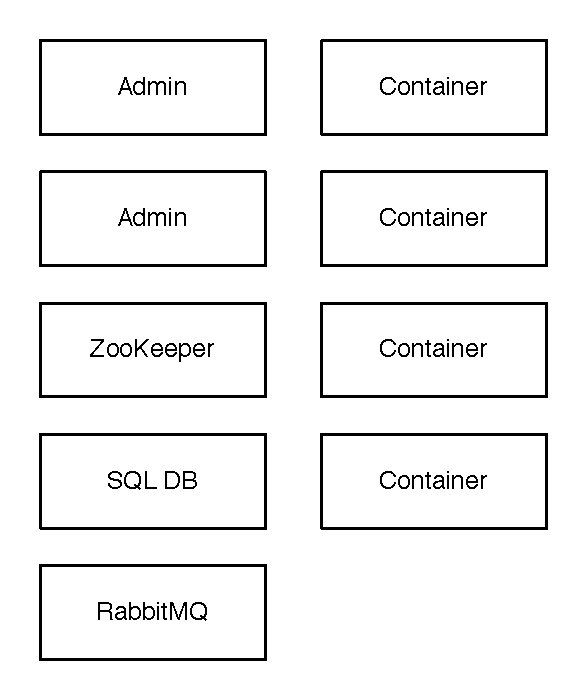
\epsfig{file=XD-sample.eps, height=2in, width=2in}
\caption{Spring XD Architecture.}
\label{fig:architecture}
\end{figure}

Here is where we get into the fine grained details.

\section{Modules}
\label{sec:Modules}
A Spring XD Module \cite{modules} is a unit of data processing. There are four module
types: source, processor, sink, and job. Modules in Spring XD are defined
in their own application context. This allows for easy encapsulation and life cycle
management for modules. Additionally, the use of an application context allows for easy
module expansion.  Spring XD uses Spring Integration \cite{spring-integration-reference}
as its foundation for implementing modules. A module is comprised of components that
implement the data processing logic and one or more connectors (known as channels)
that connect to the underlying message bus.

\par

Spring XD offers a suite of 23 sources, 24 sinks, 9 processors and 9 jobs that are ready
to use at startup.  These modules integrate with a variety of well known and popular
data stores and processing systems such as JDBC, HDFS, MongoDB, Spark, Kafka, RabbitMQ,
Sqoop, etc.  If an existing module does not meet the needs of a given use case, Spring XD
supports custom modules.

Spring XD sink and source modules are Message Endpoints
\cite{enterprise-integration-pattern-message-endpoint}
that are responsible for sending data to and receiving data from external applications
respectively. A source is the entry point for data into the stream. A sink is
the module that dispatches the stream's results to an external application or storage system.
A processor module is used to modify data transmitted from the source to sink.
Multiple processors may be chained together. Batch jobs are used to execute batch
processing steps on a set of data.

\par

\subsection{Source}
\label{sec:Source}
Source modules receive inbound data and send to downstream modules in the stream or to a batch job
which could be triggered with the data. There are two source types: poller and event driven.
A poller source is based on the polling consumer pattern \cite{enterprise-integration-pattern-pollingconsumer}.
It polls an external application (such as a web service, FTP server, database) for data at a
configurable interval. An event driven source is based on the event driven
consumer pattern \cite{enterprise-integration-pattern-eventdrivenconsumer} which
opens a port to listen for incoming data that is pushed from an external application.

\par

In the case of a source module there is an ``output'' connector channel to dispatch data
transmitted by the module to a downstream module(see figure~\ref{fig:sourcembc}.)

\par

\begin{figure}[ht]
\centering
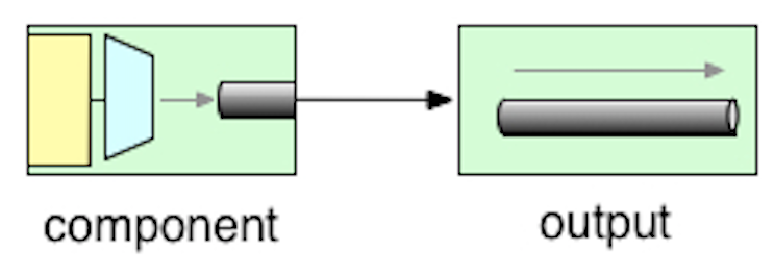
\epsfig{file=integration-module-output-channel.eps, height=.6in, width=1.75in}
\caption{Source Module Basic Components}
\label{fig:sourcembc}
\end{figure}

\par

\subsection{Processor}
\label{sec:Processor}
A processor is the module that receives data from a source or a previous processor
module's output, performs the transformation operation and sends the data
into a sink module or a downstream processor module. The basic processor
includes both ``input'' and ``output'' connector channels and the data processing component.
The input channel receives data from the upstream module and dispatches it to
the data processing component (see figure~\ref{fig:processormbc}.) It is the responsibility of
this component to transform the data. The transformed data is then sent to the downstream module
via the output channel.

\par

\begin{figure}
\centering
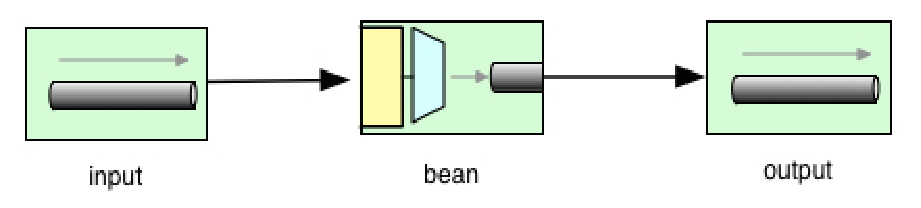
\epsfig{file=module-processor.eps, height=.6in, width=2.5in}
\caption{Processor Module Basic Components}
\label{fig:processormbc}
\end{figure}

\par

\subsection{Sink}
Sink modules convert and deliver data out of the stream in a format consumable by
an external application.  There are two types of sinks: analytic and delegate.
An analytic sink is used to perform analytic operations (such as count, gauge) on the
incoming data and store the result into a metric repository. (See section~\ref{sec:Analytics}.)
A delegate sink translates data to the format expected by the external application.
After transforming the data, the resulting data is sent to the external application.

\par

The basic sink includes an ``input'' channel connector and a data processing
component. The input channel receives data from the stream and dispatches
it to the data processing component which is responsible for connecting to the external
application(see figure~\ref{fig:sinkmbc}.) The sinks included with Spring XD have
configurable options for retries in case of failure.

\par

\begin{figure}
\centering
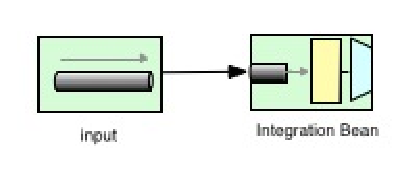
\epsfig{file=integration-module-input-channel.eps, height=.6in, width=1.75in}
\caption{Sink Module Basic Components}
\label{fig:sinkmbc}
\end{figure}

\par

\subsection{Job}
\label{sec:Job}
Spring XD uses Spring Batch \cite{spring-batch-reference}, a JSR standard (JSR-352)
for batch workload data processing as the foundation for implementing
job modules. A job enables users to execute enterprise batch processes within Spring XD.
Jobs are typically used when running long lasting tasks that have transactional requirements.
To account for failure scenarios, the workflow in the job can be designed to restart and
resume operation or roll-back the transaction altogether. A job can be triggered by the
stream with the data that act as the input to start the batch processing. This makes
streams and job modules unified under a single platform.

\par

A job typically consists of a job definition along with the supporting
data processing components as shown in figure~\ref{fig:batchmbc}.
In some cases the job definition alone is sufficient to implement the desired behavior.

\par

\begin{figure}
\centering
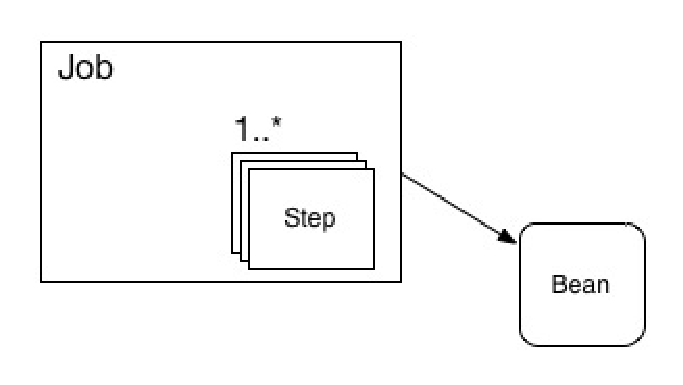
\epsfig{file=integration-batch.eps, height=.8in, width=2in}
\caption{Batch Basic Components}
\label{fig:batchmbc}
\end{figure}

\par 

\subsection{Composite}
A composite module provides a way to create a single module that contains
multiple modules. A composite module can be used to prevent
duplication when a processing chain of modules is used frequently.
Additionally, data passed between modules in a composite module will be
transmitted in memory (as opposed to the message bus) -- thus improving
performance.

\par

\subsection{Module Registry}
The module registry is where Spring XD looks for modules during
deployment. A module can be bundled as an archive or defined along with its
dependencies inside the module registry. The modules are defined in
the modules directory and are segregated in subdirectories by
type: \texttt{modules/source}, \texttt{modules/processor},
\texttt{modules/sink} and \texttt{modules/job}. The module registry is
configurable and modules may be uploaded via the admin server REST API.
During the deployment of the module, the Spring XD runtime will load the modules
dynamically from the module registry.


\section{Analytics}
\label{sec:Analytics}

Spring XD supports analytics functionality through various sink and processor modules.
Typically a ``main'' stream which obtains data from an external source (via
a source module) and writes it to an external data store (via a sink module)
is ``tapped'' -- meaning that a separate stream is created using the data
flowing from the first stream. The existence of this tap is unknown by the
main stream. This allows for analytics to be performed in a non-invasive manner.
The results of the analytics can be written to another sink module or a
subsequent processing module for further analysis.

\par

Spring XD includes analytics modules such as counter, field value counter,
aggregate counter, gauge and rich gauge. It also provides support for running
predictive analytics using PMML model scoring. Spring XD also includes a module
for executing arbitrary shell commands. This shell module can execute an R or
Python based processor or sink implementation which could perform dynamic model
scoring. Additionally, a Spark MLLib job may be executed as a Spring XD job,
benefiting from Spring XD's capability to monitor and manage the job.

\subsection {Basic Analytics}

To perform some of the basic analytic operations, Spring XD provides the following
modules. Since these modules write the analytic results to a data store, they are
considered sinks. Currently in-memory and Redis are supported data stores. This
data is exposed by the admin server via the REST API. This allows for simple
development of an application to gain access to the analytic data results.

\subsubsection {Counter}

This module counts the number of events triggered on various stages of a stream.
This can be used to tap a main stream at various stages and count the number
of messages sent out at each stage.

\subsubsection {Field Value Counter}

This module counts the number of occurrences of a specific field from a message
flowing through a stream. Spring XD supports the following message payload types
out of the box: POJO (Java Bean), Tuple and JSON string.

\subsubsection {Aggregate Counter}

The aggregate counter is similar to the simple counter but also keeps track of
the time period. Total count values for each each minute, hour, day and month
of the period in which data was collected may be queried.

\subsubsection {Gauge}
Gauge is a metric that represents a single long value associated with a unique name.
In Spring XD, the gauge metric sink expects a numeric value as a payload.

\subsubsection {Rich Gauge}
Rich Gauge is a metric that holds a double value associated with a unique name. In
addition to the value, this metric keeps a running average along with the minimum and
maximum values and the count.

\subsection {Predictive Analytics using PMML}
Spring XD provides support for running real time model scoring using JPMML-Evaluator.
This evaluator supports a wide range of model types and is interoperable with
models exported from R, Rattle, KNIME, and RapidMiner. Once the analytical model
is defined as a PMML model, the evaluator can run model scoring based on the 
input data being ingested.

\par

The Shell based processor/sink implementation can be used to run predictive
analytics algorithms written in other languages such as Python and dynamically
update the model which makes predictive analytics more adaptive.

\subsection{Spark MLLib}
A spark MLLib algorithm can be run as a sparkApp job in XD.



\section {Monitoring and Management}
Spring XD provides multiple options for management and monitoring of
its runtime components, including the following:\begin{itemize*}
	\item admin servers
	\item container servers
	\item stream and job modules
\end{itemize*}

\subsection {Monitoring via JMX and HTTP}
The runtime health, environment, and metrics information for these components
may be accessed via REST endpoints exposed by Spring Boot\cite{spring-boot}.
This functionality is also exposed via JMX; thus JMX clients such as JConsole
and Jolokia are supported.

\subsection {Management GUI}
Spring XD comes with an administrative web UI which allows users to manage
and monitor the system. The UI allows for the creation and deployment
of streams and batch jobs. Job control (start/stop) and execution status
are also supported.

\subsection {Shell Interface}
Spring XD includes an interactive shell which connects to the admin server
via the REST API. The shell exposes all of the management functionality
of the admin server.



\section{Deployment}
This section describes deployment architectures that are possible with Spring XD.
Note that this is not an exhaustive list of all deployment types. See
section~\ref{sec:Use Cases} for descriptions of real world deployments.

\subsection{Lambda Architecture}

The Lambda Architecture, introduced by Nathan Marz \cite{lambda-architecture-paper}
and shown in figure~\ref{fig:lambda}
is a generic, scalable and fault tolerant data  processing architecture. It 
attempts to provide a comprehensive solution to the problem of processing an 
extremely large set of data.

The Lambda Architecture has the following components:

\begin{itemize*}
\item A \emph{master dataset} consisting of all data known to the system,
ideally in its rawest form;
\item A \emph{serving} or \emph{view layer} that provides the latest,
most up-to-date view of the processed data, available for low-latency,
ad-hoc querying;
\item A \emph{batch layer} that performs computationally intense 
calculations and prepares the \emph{batch views} displayed by the 
\emph{serving layer};
\item A \emph{speed layer} that performs calculations on recent data only, 
its output combined with the \emph{batch views} by the \emph{serving layer}.
\end{itemize*}

The guiding principle of the Lambda architecture is to combine the
high throughput of batch operations with the low latency of real-time
computations. On its own, each has its strengths and weaknesses. While the
highest throughput for computing large datasets is reached by relying on
batch computations, the latter have the disadvantage of higher latency.
Meanwhile, real-time computations may operate with low latency and produce
results based on latest data quickly, but can't handle the large
amounts of data that batch processing can. Therefore, instead of relying
on a single paradigm, the Lambda architecture employs both, allowing them
to complement each other.

\begin{figure}[ht]
\centering
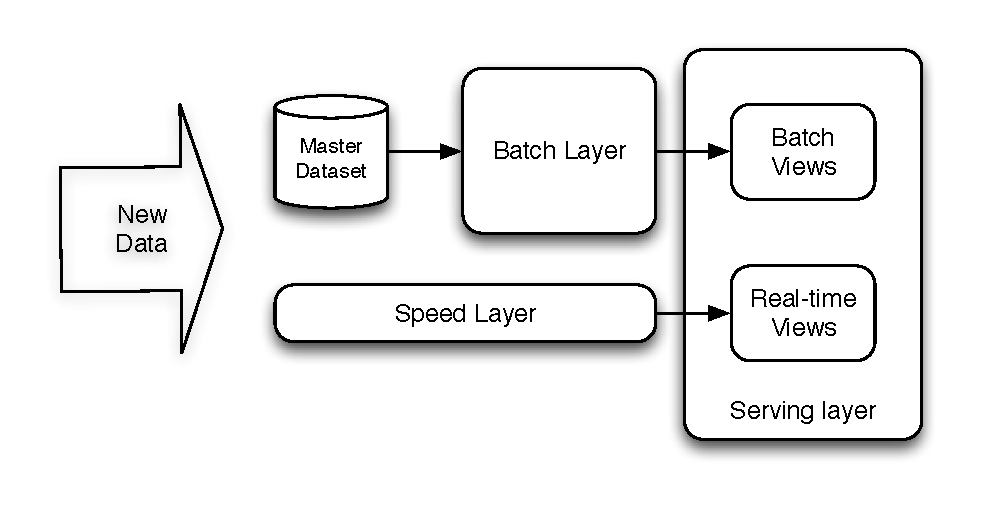
\epsfig{file=lambda.eps, height=2in, width=3in}
\caption{Lambda Architecture.}
\label{fig:lambda}
\end{figure}

In the following subsections we will examine how the different components
of the Lambda architecture can be implemented with Spring XD.

\subsubsection {Master dataset with Spring XD}

While Spring XD does not provide a storage mechanism of its own, it
integrates with a variety of storage technologies, both for reading,
via source modules (see~\ref{sec:Source}), as well as for writing, via
sink modules (see~\ref{sec:Sink}). A \emph{data ingestion}
stream can be used to consolidate data from external sources into
central storage.

For example, the following stream definition can be used to ingest 
MQTT\cite{mqtt} data sent by a number of sensors directly into HDFS:

\verb;stream create ingest --definition "mqtt | hdfs";\\*

In a more elaborate setting, an application can collect data from
different sources, and Spring XD can provide the means to merge them
in a single master dataset. The streams \texttt{in-mqtt} and \texttt{in-http}
collect data from sensors via MQTT and HTTP, respectively, and
contribute to a single queue \texttt{hdfs-in}. The merged result
is saved into HDFS.

\verb;stream create in-mqtt --definition ;\\*
\verb;  "mqtt > queue:hdfs-in";\\*

\verb;stream create in-http --definition  ;\\*
\verb;  "http > queue:hdfs-in";\\*

\verb;stream create ingest --definition  ;\\*
\verb;  "queue:hdfs-in > hdfs";\\*

\subsubsection {Batch layer in Spring XD}

Once data is collected into the \emph{master dataset}, it can be processed
by \emph{jobs} (see~\ref{sec:Job}). The similarities between Spring XD's
notion of a \emph{job} and Lambda Architecture's corresponding notion of
a \emph{batch job} make the mapping straightforward.


The data ingested in the master dataset can be consumed by a batch job,
created as follows:

\verb;job create sensorProcess;\\*
\verb;  --definition "sensors";\\*

(This example already assumes an existing module job named \emph{sensors} that
implements the processing logic).

Spring XD supports the partitioning of jobs for concurrent execution on
separate containers. This allows for increased throughput and reduced latency
for job executions. Such execution parameters are defined during deployment,
as follows:

\verb;job deploy sensor-process;\\*
\verb;  --properties module.sensorProcess.count=3;\\*

An important characteristic of the \emph{batch layer} is the regular
execution of jobs, as well as the ability to replay older datasets, for
instance for reconstructing the \emph{data views} in case of loss or error.
For that, Spring XD provides the following mechanisms:

\begin{itemize*}
\item \emph{manual} job launch through its shell user interface or 
administrative UI;
\item \emph{stream-controlled} where the jobs are lanched by stream of 
\emph{trigger} messages;
\item \emph{scheduled} job launch according to a \texttt{cron} expression;
\end{itemize*}

For example, a job can be launched manually as follows:

\verb;job launch sensor-process;\\*

Or, more typically, it can be launched on a schedule:

\verb;stream create --name launchSensorProcess;\\*
\verb;  --definition "trigger --cron='0/5 * * * * *';\\* 
\verb;  > queue:job:myCronJob" --deploy;\\*

\subsubsection {Speed layer in Spring XD}

The role of the \emph{speed layer} is to complement the \emph{batch layer} 
by performing real-time computations on the incoming data, thus filling the 
inherent latency gap. This functionality can be implemented in Spring XD by 
the its analytics support (see section~\ref{sec:Analytics}).

Considering the previous example, while ingesting data from sensors and 
populating the master dataset, the application may perform various computations 
on the data stream. For example, it can perform a count of the incoming elements. 

\verb;stream create count --definition  ;\\*
\verb;"tap:stream:ingest > aggregate-counter";\\*

In a more elaborate scenario, it is possible to actually do 
some processing of the data in-flight and store the results in real-time views
for being combined with the batch views.

\verb;stream create count --definition  ;\\*
\verb;"tap:stream:ingest > extract-tags | jdbc";\\*

\subsubsection {Serving layer with Spring XD}

Spring XD provides out-of-the box RESTful services for its counters and gauges,
which can operate as part of the serving layer. In addition to that,  
the data stored by the \emph{batch jobs} in the 
\emph{batch views}, as well as \emph{real time views} produced by the streams, 
can be easily made availabe through a serving layer using Spring Boot \cite{spring-boot}, 
in combination with Spring Data \cite{spring-data} or Spring Data REST \cite{spring-data-rest}.

\subsection {Reactive applications}

The last few years have seen a significant change in application requirements:
data volumes of terabyte order, response times within tens of milliseconds, stricter
availability requirements. These new challenges require a new approach to application
development, subsumed under the concepts of \emph{reactive applications} and \emph{reactive
programming}. In what follows next, we will describe how these concepts are
illustrated by Spring XD, both from a runtime platform, as well as from a development perspective.

\subsubsection {Spring XD as a platform for reactive applications}

Reactive applications, as described by the Reactive Manifesto
\cite{reactive-manifesto} are \emph{responsive},\emph{resilient},\emph{elastic}
and \emph{message-driven}. Spring XD, as a platform, provides the means for creating and
running reactive applications.

\emph{Responsiveness} represents system's ability to respond in a timely manner, if
at all, possible. In the case of Spring XD, its stream processing model is designed
for building fast, low-latency data pipelines.

\emph{Resilience} represents a system's ability to remain responsive in the face of
failure. In Spring XD, this is provided out of the box by features such as automatic
module redeployment if the host container has crashed, or the ability to elect a new
admin node in case the existing one fails. On a more granular level, automatic retry
and dead-letter queue support for RabbitMQ and Redis allows tracking and recovery
from failed computations. The use of messaging middleware ensures redelivery of data
when a module recovers.

\emph{Elasticity} represents a system's ability to remain responsive under varying
workload. In Spring XD, this is provided by features such as the ability to scale up
the processing power by deploying multiple instances of a module or job in a stream.
The use of messaging middleware provides backpressure allowing each component in the
stream to consume data at its own pace.

\emph{Message-driven} represents a system's reliance on asynchronous message passing
between components. This is a core feature of Spring XD, implemented by its
message bus (see~\ref{subsec:MessageBus}).

This is how Spring XD as a platform allows applications to meet the criteria for being
considered \emph{reactive}. In conjunction with that, it provides the ability of using
a development model that is better suited for reactive applications, through its support
for \emph{reactive programming} and \emph{observable streams}.

\subsubsection {Reactive programming and functional in Spring XD}

\emph{Reactive programming} is a programming paradigm centered around asynchronous stream processing. The central
notion is that incoming data can be processed in an ordered, asynchronous and event-driven manner, using functional
operators to describe transformations that apply to an entire stream of incoming data. The operators can vary from
individual item transformations, to grouping and aggregation over given time windows, and can be composed into 
complex data processing pipelines that produce outbound streams of data. 

ReactiveX~\cite{reactivex} is one of the most common set of APIs, centered around the \texttt{Observable} abstraction that
extends the observer pattern to streams, together with a rich set of operators for composing and transforming sequences, and
RxJava~\cite{rxjava} is the Java implementation of the ReactiveX API. Another reactive programming library for Java is provided
by Project Reactor~\cite{projectreactor}, whose abstraction is called a \texttt{Stream}. Reactive Streams~\cite{reactivestreams} is an initiative 
to provide a standard for asynchronous stream processing with non-blocking backpressure (the ability of the consumers to regulate
the data flow and instruct the producers to adjust their production rate) on the JVM.

Spring XD provides support for reactive programming through a special type of processors that transform asynchronous streams of 
data. Both the APIs for RxJava and Project Reactor are supported. An example of an RxJava processor is shown in figure \ref{fig:rxjava}, and 
Reactor integration is almost identical. Spring XD has the responsibility of transforming the flow of discrete messages arriving on processor's input channel into an RxJava \texttt{Observable}, as well as transforming the \texttt{Observable} returned by the processor module into a flow of discrete messages sent on the output channel. Inside the processor, RxJava operators are applied for performing transformations on the data stream. 

\begin{figure}[ht]
\centering
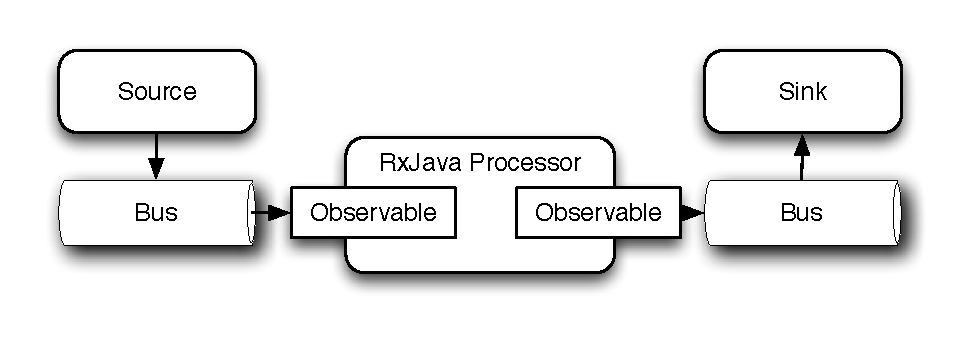
\epsfig{file=rxjava.eps, height=2in, width=3in}
\caption{Reactive module using RxJava}
\label{fig:rxjava}
\end{figure}



\section{Use Cases}
The following customer use cases are being supported in the field by the Spring XD team.

\begin{itemize*}
\item \textbf{Fault Detection}: \textit{Challenge}: A large equipment manufacturer is  interested in ingesting machine data to apply predictive analytics to proactively monitor performance and adjust business operations. \textit{Solution}: Given the extensible architecture in Spring XD, a custom source module was created to handle proprietary data formats, thus allowing consumption and transformation of data complying with their proprietary standards. The predictive models, complying with PMML specification, were generated based on historical trends. Spring XD's analytic-pmml processor was used in a stream to intercept machine events to compute predictions in real-time. The outliers were captured in Redis for dashboard alerts and ad-hoc data analysis via REST.
\item \textbf{Enterprise Modernization}: \textit{Challenge}: A large retail provider is heavily invested in Hadoop ecosystem. They weren't keen on maintaining or supporting several products in production - operationalizing this was painful. They wanted to streamline and modernize their Hadoop workflows. \textit{Solution}: As one-stop runtime, Spring XD provides dozens of data integration adapters to send and receive data from external applications, thus allowing the customer to use the unified approach for all ingestion use-cases. Building upon Spring Batch, Spring XD also provides multiple batch jobs for data movements along with granular workflow steps. This further eliminated the need for relying on different workflow and data movement tools. Whether it is MapReduce, Hive, Pig, or HBase scripts - developer experience is the same.
\item \textbf{Data Ingest}: \textit{Challenge}: A startup in San Francisco was looking for a solution to unify stream and batch operations. \textit{Solution}: Spring XD is used as a standard tool for ingesting data into Hadoop. Whether it is real-time (i.e., online) or batch (i.e., offline), the out of the box fixtures delivered immediate benefits. Overall, the data integration, orchestration, and data movement capabilities were handled end to end by Spring XD.
\item \textbf{24/7 Production Pipelines}: \textit{Challenge}: A large IT enterprise wanted to build data pipelines to monitor current software and hardware sales in order to predict and forecast. Building pipelines in one; running them reliably 24/7 with strict SLAs is another big challenege. \textit{Solution}: Spring XD is built as highly-available runtime. Automatic recovery from fault sceanrios along with reproccessing of data events fulfilled SLAs guarantees. Production running pipelines in Spring XD are long-running processes. For ad-hoc operations such as querying, machine learning, or data crunching, `taps' in Spring XD were adopted to fork the data from primary pipeline. This results in no disruption with the primary pipeline, at the same time satisfying ad-hoc demands.
\item \textbf{Closed-loop Analytics}: \textit{Challenge}: A finance institution wanted to build a platform to detect fraudulent transactions. They had years of historical data in varying formats and the transactions happening in real-time at high volume. They wanted to automate generation of historical models from raw dataset and apply the models to real-time events. No in-house talent to build one; neither had budget to buy expensive products. \textit{Solution}: A batch job was used to learn from historical data thus producing predictive models complying with PMML specification. The last step in the batch workflow is orchestrated to deliver the generated models to streams that ingest for real-time predictions. The predictions were persisted in in-memory data grids to feed the dashboard. Spring XD, thus eliminating top-talent hires to operationalize analytics pipeline.
\end{itemize*}

\section{Related Work}
This section compares and contrasts Spring XD to similar projects.

\subsection{Spark}
\label{sec:Spark}
Apache Spark is a general purpose framework for large scale data processing.
In comparison with Hadoop's disk based MapReduce programming model, Spark's
in-memory primitives yields performance improvements.

The following features differentiate Spring XD and Spark Streaming.

\begin{itemize*}
\item Ability to microbatch based on event count via Reactor and RxJava APIs.
\item Ability to create data pipelines to process one event at a time.
\item Flexibility to specify hosts to dictate the location of data computations.
\end{itemize*}

The following features differentiate Spring XD and Spark Batch processing.

\begin{itemize*}
\item Provides REST-API and lifecycle management for Spark jobs.
\item Extensible to integrate with other batch systems.
\end{itemize*}

Recognizing the strengths of distributed data computations with Spark, Spring XD
supports integration with Spark applications such as Spark Streaming, MLLib, and
SparkSQL. Users familiar with Spark may implement the computation logic using
Spark APIs in Java or Scala, and leave the orchestration to Spring XD.

\subsubsection{Integration with any Spark application}
A Spark Application can be deployed and launched from Spring XD as
a \emph{batch} job. A Spring XD batch job submits the Spark application into
Spark cluster manager using org.apache.spark.deploy.SparkSubmit. One advantage 
of this approach is that one can launch a Spark application with specific criteria
via Spring XD stream. For instance, a real time scoring algorithm through Spark MLlib
job can be triggered based on the criteria from a regular \emph{XD stream} events. 
Another advantage is after the job is complete a notification can be sent to a 
stream for processing.

\subsubsection{Integration with Spark Streaming}
 Spring XD integrates with Spark streaming to provide better orchestration and
lifecycle management for spark streaming applications. Spring XD runs the
Spark Driver as an -- XD module (processor or sink) in the XD container
while the \emph{spark streaming receiver} and subsequent \emph{data computation} is
done at the \emph{Spark Cluster}. Driver failure is automatically handled by
Spring XD -- the admin server will re-deploy a module from a failed container
to another eligible container.
 Setting up a Spark Streaming module within XD can be beneficial when adding
streaming data computation logic for a tapped XD stream. While the primary
stream processes events one at a time (through the regular XD modules),
the tapped stream will become a source for the Spark Streaming module.

\subsection{Storm}
Apache Storm\cite{storm} is a distributed computation system for real time stream
processing.

The following features differentiate Spring XD and Storm.

\begin{itemize*}
\item Spring XD provides an interactive shell while Storm requires programming
to an API to create data pipelines.
\item Use of \emph{taps} in Spring XD allows the creation of stream pipelines
in isolation without having to disrupt existing pipelines.
\item Loosely coupled modules in Spring XD are responsible for ingestion, analytics,
data processing, machine learning or data export. Modules can be individually managed
and dynamically scaled. Additionally modules may be co-located to minimize
serialization and network usage.
\item Building upon the functional stream processing model, users have the option
to choose from Reactor\cite{reactor}, Spark Streaming or RxJava APIs to build
complex data centric applications.
\item As an alternative to linear streaming data pipelines, Spring XD provides
support for directed graphs through named channels to combine multiple flows
upstream or downstream from the message channel. The behavior of the channel
can be either queue-based on topic-based. However, Storm accepts Directed
Acyclic Graph (DAG)\cite{dag} of operations that represent streaming
computations.
\end{itemize*}

Here is a Spring XD example that shows how you can use a named channel to share
a data pipeline driven by different input sources.

\begin{lstlisting}
queue:foo > file
http > queue:foo
time > queue:foo
\end{lstlisting}

Now if you post data to the http source, you will see that data intermingled
with the time value in the file.

\begin{lstlisting}
tap:stream:mystream > file
tap:stream:mystream > log
\end{lstlisting}

Storm and Spring XD support many common data sources and middleware;
for example, the reading and writing of data payloads from Apache Kafka
is supported in both. A Spout in Storm is analogous to a
source in Spring XD, and Bolts in Storm are similar to processors and sinks
in Spring XD. As stream processing frameworks, Storm and Spring XD can be used for
similar use-cases.

\subsection{Samza}
Apache Samza\cite{samza} is a distributed stream processing framework that uses
Kafka for messaging and YARN for fault-tolerance and other non-functional
requirements.

The following features differentiate Spring XD and Samza.

\begin{itemize*}
\item Spring XD provides sources and sinks for reading and writing to a 
variety systems, while Samza requires the end user to provide their
own implementations, using Samza's API.
\item Spring XD's runtime abstraction allows extensions and additional
customizations. Though extensible, the implementation in Samza should comply with
Samza-compatible streaming system, which generally means it is very much Kafka
or similar.
\item Spring XD provides built-in fault-tolerance, security, and logging; whereas,
Samza relies on YARN to support non-functional requirements.
\item Spring XD's YARN support provides cluster/group semantics, which allows
ramping up/down and also creating such groups dynamically. The container `count'
in Samza is static - requires redeployment to rebalance scaling of containers.
\end{itemize*}

Samza offers local-state repository with the option of log-backed replication,
which could be desirable as a standalone general purpose resilient cache.

\subsection{Flume}
Apache Flume\cite{flume} is a distributed system for collecting, aggregating and
moving large data sets.

The following features differentiate Spring XD and Flume.

\begin{itemize*}
\item Spring XD uses an interactive shell and DSL for stream creation,
while Flume uses property (key/value pair) files.
\item Administration and monitoring via the admin UI.
\item Granular controls to manifest batch job and step execution to create
complex data driven workflows.
\item Flexibility through a deployment manifest to declaratively configure data
partitioning strategy to route data to a specific consumer instance in the cluster.
\end{itemize*}

Flume offers HBase, Solr, and ElasticSearch sinks along with encryption support
for Avro sources, which we are planning to address in our future releases.

\subsection{Oozie}
Apache Oozie\cite{oozie} is a workflow scheduler engine to manage Hadoop \cite{hadoop}
workloads such as MapReduce or Pig jobs.

The following features differentiate Spring XD and Oozie.

\begin{itemize*}
\item Building upon Spring Batch, a JSR standardization (JSR-352) of batch
workload data processing, Spring XD inherits workflow scheduling and execution
functionalities.
\item Provides out of the box batch jobs that support plain files, JDBC, HDFS,
FTP, MongoDB, Spark and Sqoop.
\item Ability to scale jobs without having to bring down the runtime.
\item Provides bi-directionality between real-time streaming and batch
workflows to accommodate complex data processing use cases.
\item Ability to create, and launch jobs from the admin UI.
\item Ability to view historical snapshots of job executions from the admin UI.
\end{itemize*}

Oozie offers HCatalog integration, which we are planning to address in our
future releases.

\subsection{Sqoop}
Apache Sqoop\cite{sqoop} assists with data transmission between Hadoop and relational
databases.

The following features differentiate Spring XD and Sqoop.

\begin{itemize*}
\item Ability to orchestrate Pig, Hive, HBase, MapReduce or other batch systems.
\item Flexibility to extend and customize batch workflow infrastructure.
\item High level configuration DSL to create, deploy and destroy batch workflows.
\item Flexibility to operationalize custom data pipelines through REST.
\item Unified functional programming support to build reactive-style data pipelines.
\end{itemize*}

Sqoop offers data validation and HCatalog integration among others. Recognizing the
importance of these enterprise features, Spring XD provides an out of the box Sqoop
job to take advantage of these features.


\section{Conclusion}

Mission critical data applications cannot live in a vacuum. The abundance of data
and specialized applications to process and store it require a holistic approach.
Spring XD is a formidable solution for managing the data flow and processing
between these applications. Spring XD integrates with systems ranging from decades
old RDBMS to cutting edge Big Data. The suite of Spring Framework projects that
Spring XD builds upon allows for flexible extensibility. The distributed runtime
built on ZooKeeper provides reliability and scale out capabilities for streams
and jobs. 


%\end{document}  % This is where a 'short' article might terminate

%ACKNOWLEDGMENTS are optional
%\section{Acknowledgments}
%This section is optional; it is a location for you
%to acknowledge grants, funding, editing assistance and
%what have you.  In the present case, for example, the
%authors would like to thank Gerald Murray of ACM for
%his help in codifying this \textit{Author's Guide}
%and the \textbf{.cls} and \textbf{.tex} files that it describes.

%
% The following two commands are all you need in the
% initial runs of your .tex file to
% produce the bibliography for the citations in your paper.
\bibliographystyle{abbrv}
\bibliography{spring-xd}  % sigproc.bib is the name of the Bibliography in this case
% You must have a proper ".bib" file
%  and remember to run:
% latex bibtex latex latex
% to resolve all references
%
% ACM needs 'a single self-contained file'!
%

% This next section command marks the start of
% Appendix B, and does not continue the present hierarchy
\balancecolumns
% That's all folks!
\end{document}
